% This is a Basic Assignment Paper but with like Code and stuff allowed in it. 

\documentclass[11pt]{article}

% Preamble

\usepackage[margin=1in]{geometry}
\usepackage{amsfonts, amsmath, amssymb}
\usepackage{fancyhdr, float, graphicx}
\usepackage[utf8]{inputenc} % Required for inputting international characters
\usepackage[T1]{fontenc} % Output font encoding for international characters
\usepackage{fouriernc} % Use the New Century Schoolbook font
\usepackage[nottoc, notlot, notlof]{tocbibind}
\usepackage{listings}
\usepackage{xcolor}

\definecolor{codegreen}{rgb}{0,0.6,0}
\definecolor{codegray}{rgb}{0.5,0.5,0.5}
\definecolor{codepurple}{rgb}{0.58,0,0.82}
\definecolor{backcolour}{rgb}{0.95,0.95,0.92}

\lstdefinestyle{mystyle}{
    backgroundcolor=\color{backcolour},   
    commentstyle=\color{codegreen},
    keywordstyle=\color{magenta},
    numberstyle=\tiny\color{codegray},
    stringstyle=\color{codepurple},
    basicstyle=\ttfamily\footnotesize,
    breakatwhitespace=false,         
    breaklines=true,                 
    captionpos=b,                    
    keepspaces=true,                 
    numbers=left,                    
    numbersep=5pt,                  
    showspaces=false,                
    showstringspaces=false,
    showtabs=false,                  
    tabsize=2
}

\lstset{style=mystyle}

% Header and Footer
\pagestyle{fancy}
\fancyhead{}
\fancyfoot{}
\fancyhead[L]{\textit{\Large{OOPJC Assignment 4}}}
%\fancyhead[R]{\textit{something}}
\fancyfoot[C]{\thepage}
\renewcommand{\footrulewidth}{1pt}



% Other Doc Editing
% \parindent 0ex
%\renewcommand{\baselinestretch}{1.5}

\begin{document}

\begin{titlepage}
	\centering

	%---------------------------NAMES-------------------------------

	\huge\textsc{
		MIT World Peace University
	}\\

	\vspace{0.75\baselineskip} % space after Uni Name

	\LARGE{
		Object Oriented Programming with Java and C++\\
		Second Year B. Tech, Semester 1
	}

	\vfill % space after Sub Name

	%--------------------------TITLE-------------------------------

	\rule{\textwidth}{1.6pt}\vspace*{-\baselineskip}\vspace*{2pt}
	\rule{\textwidth}{0.6pt}
	\vspace{0.75\baselineskip} % Whitespace above the title



	\huge{\textsc{
			Developing a Simple Graphical Calculator using Swing in Java
		}} \\



	\vspace{0.5\baselineskip} % Whitespace below the title
	\rule{\textwidth}{0.6pt}\vspace*{-\baselineskip}\vspace*{2.8pt}
	\rule{\textwidth}{1.6pt}

	\vspace{1\baselineskip} % Whitespace after the title block

	%--------------------------SUBTITLE --------------------------	

	\LARGE\textsc{
		Practical Report\\
		Assignment 8
	} % Subtitle or further description
	\vfill

	%--------------------------AUTHOR-------------------------------

	Prepared By
	\vspace{0.5\baselineskip} % Whitespace before the editors

	\Large{
		Krishnaraj Thadesar \\
		Cyber Security and Forensics\\
		Batch A1, PA 20
	}


	\vspace{0.5\baselineskip} % Whitespace below the editor list
	\today

\end{titlepage}


\tableofcontents
\thispagestyle{empty}
\clearpage


\setcounter{page}{1}

\section{Aim and Objectives}
\subsection*{Aim}
To Develop a simple calculator using Swing in Java
\subsection*{Objective}
\begin{enumerate}
	\item To understand concept of AWT and Java swings
	\item To explore Java Swing containers
\end{enumerate}
\section{Problem Statement}
Write a Java program to create a simple calculator with the help of java swing.

\section{Theory}
% Java Swing containers
% 
%  Container classes of Java Swing with examples
% 
%  Swing components including buttons, checkboxes, sliders, and list boxes, etc.
% 
%  Heavyweight Components and Lightweight Components
% 
%  What is Double Buffering?
% 
%  Difference between applet and Swing
\section{Platform}
\textbf{Operating System}: Arch Linux x86-64 \\
\textbf{IDEs or Text Editors Used}: Visual Studio Code\\
\textbf{Compilers} : g++ and gcc on linux for C++, and javac, with JDK 18.0.2 for Java\\

\section{Input}
The numbers and the Operators.

\section{Output}
The Output of the entered Calculation in the Display Section of the Calculator
\begin{figure}[H]
	\centering
	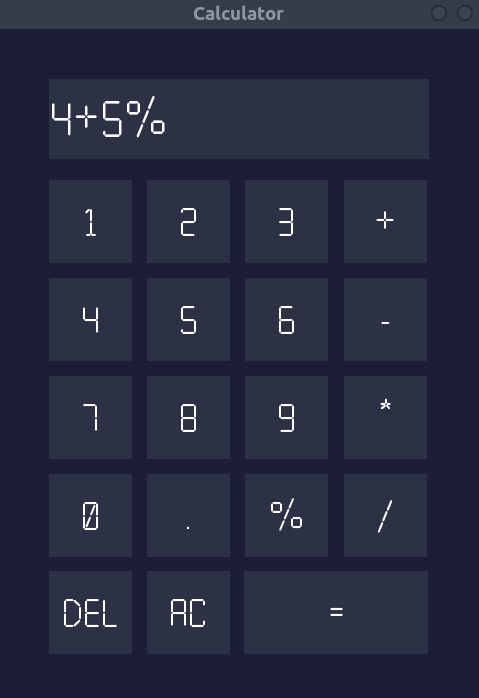
\includegraphics[scale=0.5]{Calculator.png}
	\caption{Calculator with Java Swing}
\end{figure}

\section{Code}

\lstinputlisting[language=java, caption=Calculator.java]{../Programs/java_implementations/assignment_8/Calculator/src/main/java/org/OOPCJ/Krishnaraj/Main.java}

\section{Dependencies}
\lstinputlisting[language=java, caption=pom.xml]{../Programs/java_implementations/assignment_8/Calculator/pom.xml}
	
\section{Conclusion}
Thus, implemented simple calculator with the help of java swing and performed various
operations.

\pagebreak

\section{FAQs}
\begin{enumerate}
	\item \textit{What are the methods of component class in Java Swing?}

	\item \textit{How many ways to create a frame in Java Swing? Explain with examples}

	\item \textit{What are the methods of JLabel class in Java Swing?}

	\item \textit{What are the methods of AbstractButton class in Java Swing?}

	\item \textit{Write a simple Java Swing program of displaying image on the button?}

\end{enumerate}

\end{document}